\section{Separability}

  Separability comes in different levels.\footnote{Note that this is not to be confused with the separation of a space, which is a completely different topological property.} We briefly define some weaker forms of separability. 
  
  \begin{definition}[$t_0$-Separability]
    A topological space $X$ is said to be \textbf{$t_0$-separable} if for each pair of distinct points $x, y \in X$, there exists a neighborhood $U$ that contains $x$ but not $y$, or a $U$ that contains $y$ but not $x$. 

    \begin{figure}[H]
      \centering 
      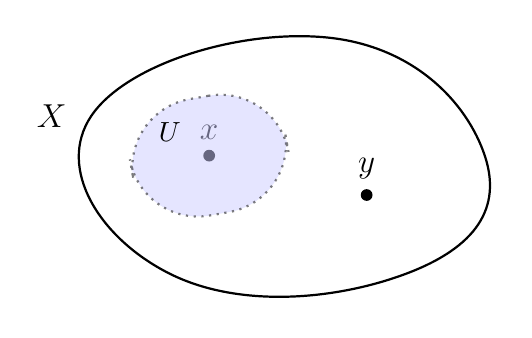
\begin{tikzpicture}[
          point/.style={circle, fill, inner sep=1.5pt},
          set/.style={draw, dotted, thick, rotate=10, minimum width=2cm, minimum height=1.5cm, rounded corners=25pt},
          mylabel/.style={font=\large\itshape}
      ]
        % Draw the topological space X
        \draw[thick] plot [smooth cycle, tension=0.8] coordinates {(0,0) (3,1) (5,-0.5) (4,-2) (1,-2)};
        \node[font=\large] at (-0.5,0) {$X$};
        
        % Draw the points
        \node[point, label={[mylabel]above:$x$}] (x) at (1.5,-0.5) {};
        \node[point, label={[mylabel]above:$y$}] (y) at (3.5,-1) {};
        
        % Draw only one open neighborhood (T0 only requires one direction)
        \node[set, fill=blue!20, opacity=0.5] (Ux) at (x) {};
        
        % Label the neighborhood
        \node[font=\normalsize] at (1,-0.2) {$U$};
      \end{tikzpicture}
      \caption{$t_0$-separability. } 
      \label{fig:t0_separability}
    \end{figure}
  \end{definition}

  \begin{example}[Nested Interval Topology is Not $t_0$]
    $(0,1)$ with the nested interval topology is not $t_0$-separable, since we can't distinguish $\frac{1}{4}$ and $\frac{1}{3}$.
  \end{example}

\subsection{T1 Separability}

  \begin{definition}[$t_1$-Separability]
    A topological space $X$ is said to be \textbf{$t_1$-separable} if for each pair of distinct points $x, y \in X$, we can find two neighborhoods $U_x, U_y$ where $y \not\in U_x$ and $x \not\in U_y$. 

    \begin{figure}[H]
      \centering 
      \begin{tikzpicture}[
        point/.style={circle, fill, inner sep=1.5pt},
        set/.style={draw, dotted, thick, rotate=10, minimum width=2cm, minimum height=1.5cm, rounded corners=25pt},
        mylabel/.style={font=\large\itshape}
      ]
        % Draw the topological space X
        \draw[thick] plot [smooth cycle, tension=0.8] coordinates {(0,0) (3,1) (5,-0.5) (4,-2) (1,-2)};
        \node[font=\large] at (-0.5,0) {$X$};
        
        % Draw the points
        \node[point, label={[mylabel]above:$x$}] (x) at (1.5,-0.5) {};
        \node[point, label={[mylabel]above:$y$}] (y) at (3.5,-1) {};
        
        % Draw the open neighborhoods with significant overlap (to show T1 is weaker than Hausdorff)
        \node[set, fill=blue!20, opacity=0.5] (Ux) at ($(x) + (0.6,0)$) {};
        \node[set, fill=red!20, opacity=0.5] (Uy) at ($(y) + (-0.6,0)$) {};
        
        % Label the neighborhoods
        \node[font=\normalsize] at (0.7,0) {$U_x$};
        \node[font=\normalsize] at (4.2,-0.3) {$U_y$};
        
        % Add annotation to clarify that in T1, x ∉ Uy and y ∉ Ux 
        \node[font=\small, align=center] at (0.5,-1.5) {$y \notin U_x$};
        \node[font=\small, align=center] at (5,-1.5) {$x \notin U_y$};
      \end{tikzpicture}
      \caption{$t_1$-separability. } 
      \label{fig:t1_separability}
    \end{figure}
  \end{definition}

  \begin{definition}
    One point sets are closed is the $T_1$ axiom. Equivalently, for any pair $x_1 \neq x_2$, there is an open set $U$ s.t. $x_1 \in U$ and $x_2 \not\in U$. 
  \end{definition}

  \begin{example}[Cofinite is $t_1$]
    $(0,1)$ with the cofinite topology is $t_0$-separable, since given distinct $x_1, x_2 \in (0,1)$, we can see that $x_1 \in X \setminus {x_2}$ and $x_2 \in X \setminus {x_1}$, which are both elements of the cofinite topology. By existence of these elements, $(0,1)$ is $t_1$-separable. 
  \end{example}

\subsection{Preservation of T1 Separability}

\subsection{T2 Hausdorff Spaces}

  Generally, mathematicians consider the Hausdorff condition as a mild extra conditions on topological spaces that make it much easier to deal with. We will assume that most of the topological spaces we work with are Hausdorff. 

  \begin{definition}[Hausdorff Space]
    A topological space $X$ is called a \textbf{Hausdorff space}, or \textbf{$t_2$-separable}, if for each pair of distinct points $x, y \in X$, there exists neighborhoods $U_x, U_y$ that are disjoint.

    \begin{figure}[H]
      \centering 
      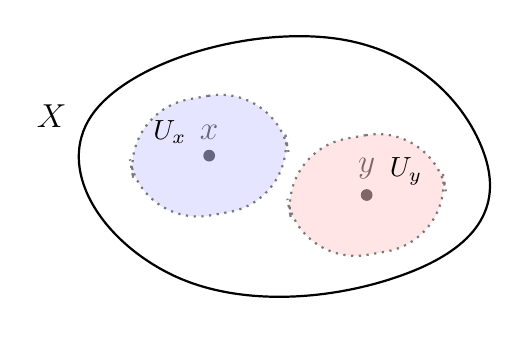
\begin{tikzpicture}[
          point/.style={circle, fill, inner sep=1.5pt},
          set/.style={draw, dotted, thick, rotate=10, minimum width=2cm, minimum height=1.5cm, rounded corners=25pt},
          mylabel/.style={font=\large\itshape}
      ]
        % Draw the topological space X
        \draw[thick] plot [smooth cycle, tension=0.8] coordinates {(0,0) (3,1) (5,-0.5) (4,-2) (1,-2)};
        \node[font=\large] at (-0.5,0) {$X$};

        % Draw the points
        \node[point, label={[mylabel]above:$x$}] (x) at (1.5,-0.5) {};
        \node[point, label={[mylabel]above:$y$}] (y) at (3.5,-1) {};

        % Draw the open neighborhoods
        \node[set, fill=blue!20, opacity=0.5] (Ux) at (x) {};
        \node[set, fill=red!20, opacity=0.5] (Uy) at (y) {};

        % Label the neighborhoods
        \node[font=\normalsize] at (1,-0.2) {$U_x$};
        \node[font=\normalsize] at (4,-0.7) {$U_y$};
      \end{tikzpicture}
      \caption{Every pair of distinct points must satisfy this separability condition in a Hausdorff space.} 
      \label{fig:hausdorff}
    \end{figure}
  \end{definition}

  \begin{theorem}[Limit Points in Hausdorff Spaces]
    Given Hausdorff space $X$ and subset $A \subset X$ a point $x$ is a limit point of $A$ if and only if every neighborhood of $x$ contains infinitely many point of $A$. It immediately follows that every finite point set in a Hausdorff space $X$ is closed. 
  \end{theorem}
  \begin{proof}
    We prove both directions
    \begin{enumerate}
      \item $(\rightarrow)$ Assume that $x$ is a limit point of $A$ with some neighborhood $U_x$ intersecting $A$ in finitely many points. Then, let the points of intersections be 
      \begin{equation}
        \{x_1, ..., x_n\} = A \cap \{U_x \setminus \{x\} \}
      \end{equation}
      But $U_x \setminus \{x\}$ is open $\implies H \coloneqq \{U_x \setminus ( \{x\} \cup \{x_1, ..., x_n\})\}$ is open. But $H \cap A = \emptyset$, contradicting the assumption that $x$ is a limit point. 

      \item $(\leftarrow)$ Simple. 
    \end{enumerate}
    It suffices to show that every one point set $\{x_0\}$ is closed. If $x$ and $x_0$ are distinct points, then by definition of Hausdorff spaces they have disjoint neighborhoods $U_x$ and $U_{x_0} \implies x \not\in \bar{\{x_0\}} \implies \{x_0\} = \bar{\{x_0\}}$, so $\{x_0\}$ is closed. 
  \end{proof}

  \begin{lemma}[Product of Hausdorff Spaces]
    Arbitrary Cartesian products of Hausdorff spaces is Hausdorff.\footnote{Since this is in the product topology, it immediately follows that the product is also Hausdorff in the finer box topology.}
  \end{lemma}

  \begin{lemma}[Subspaces of Hausdorff Spaces]
    A subspace of a Hausdorff space is Hausdorff. 
  \end{lemma}

  \begin{theorem}[Unique Point of Convergence]
    If a sequence converges in a Hausdorff space $X$, it converges to one point. 
  \end{theorem}
  \begin{proof}
    For if $(x_\alpha)$ converges to $x$ and if $y \neq x$, then we need only choose disjoint neighborhoods of $y$ and $x$ to prove that $(x_\alpha)$, by definition, is not convergent to $y$.
  \end{proof}

  \begin{example}
    The space $(0,1)$ with the nested interval topology is not Hausdorff. In fact, it is impossible to distinguish 2 points $x, y$ if $x, y \in (0, \frac{1}{2})$, meaning that the sequence
    \begin{equation}
        \frac{1}{10}, \frac{2}{10}, \frac{1}{10}, \ldots
    \end{equation}
    converges to both $\frac{1}{10}$ and $\frac{2}{10}$.
  \end{example} 

  \begin{theorem}
    Every metric topology satisfies the Hausdorff Axiom.
  \end{theorem}
  \begin{proof}
    If $x$ and $y$ are distinct points of $(X, d)$, then letting
    \begin{equation}
      \varepsilon = \frac{1}{2} d(x, y)
    \end{equation}
    the triangle inequality implies that $B_\varepsilon (x)$ and $B_\varepsilon (y)$ are disjoint. 
  \end{proof}

  \begin{lemma} 
    $X$ Hausdorff implies any finite subset is closed. 
  \end{lemma}

  \begin{example}
    $X$ is an infinite set, then finite complement topology is not Hausdorff. 
  \end{example} 

  \begin{example}[Line with Two Origins]
    $X = \mathbb{R} \setminus \{0\} \cup \{0_1, 0_2\}$ with basis given by intervals $(a, b)$ for $b < 0$ or $a > 0$, and $(a, 0) \cup \{0_i\} \cup (0, b)$ for $a < 0 < b$. 
  \end{example}

\subsection{Preservation of Hausdorff}

\subsection{Regular Spaces}

  \begin{definition}[Regular Spaces]
    Suppose that one-point sets are closed in $X$. Then, $X$ is said to be \textbf{regular}, or \textbf{$t_3$-separable}, if for each pair consisting of a point $x$ and a closed set $C$ disjoint from $x$, there exist disjoint open sets containing $x$ and $C$, respectively. 

    \begin{figure}[H]
      \centering 
      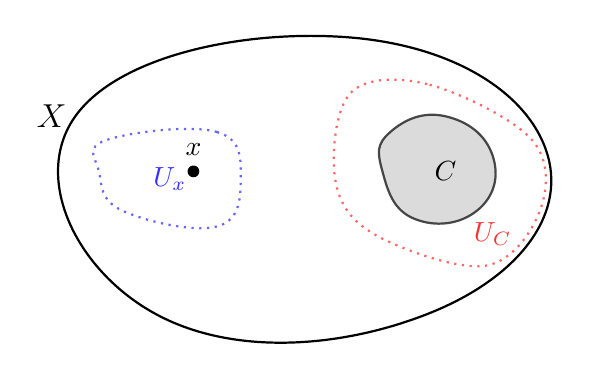
\begin{tikzpicture}[
          point/.style={circle, fill, inner sep=1.5pt},
          closed/.style={draw, thick, fill=gray!40, opacity=0.7},
          open/.style={draw, dotted, thick}
      ]

      % Draw the topological space X
      \draw[thick] plot [smooth cycle, tension=0.8] coordinates {(0,0) (3.5,1) (6,-0.5) (4.5,-2.5) (1,-2.5)};
      \node[font=\large] at (-0.3,0) {$X$};

      % Draw the point x
      \node[point, label={[font=\itshape]above:$x$}] (x) at (1.5,-0.7) {};

      % Draw the closed set C
      \draw[closed] plot [smooth cycle, tension=0.8] coordinates {(4,-0.2) (4.7,0) (5.3,-0.5) (5.1,-1.2) (4.3,-1.3) (3.9,-0.7)};
      \node at (4.7,-0.7) {$C$};

      % Draw the open set containing x
      \draw[open, blue!60, thick] plot [smooth cycle, tension=0.7] coordinates {(0.4,-0.3) (1.8,-0.2) (2.1,-0.8) (1.8,-1.4) (0.6,-1.2) (0.3,-0.7)};
      \node[blue!80] at (1.2,-0.8) {$U_x$};

      % Draw the open set containing C
      \draw[open, red!60, thick] plot [smooth cycle, tension=0.6] coordinates {(3.5,0.3) (4.5,0.4) (5.8,-0.3) (5.9,-1.2) (5.2,-1.9) (3.8,-1.5) (3.3,-0.8)};
      \node[red!80] at (5.3,-1.5) {$U_C$};

      \end{tikzpicture}
      \caption{Regular space.} 
      \label{fig:regular}
    \end{figure}

  \end{definition}

  \begin{lemma}[Product of Regular Spaces]
    Arbitrary Cartesian products of regular spaces is regular. 
  \end{lemma}

  \begin{lemma}[Subspaces of Regular Spaces]
    A subspace of a regular space is regular.  
  \end{lemma}

\subsection{Preservation of Regularity}

\subsection{Normal Spaces}

  \begin{definition}[Normal Spaces]
    Suppose that one-point sets are closed in $X$. Then, $X$ is said to be \textbf{normal}, or \textbf{$t_4$-separable}, if for each pair $C, D$ of disjoint closed sets of $X$, there exist disjoint open sets containing $C$ and $D$, respectively. 

    \begin{figure}[H]
      \centering 
      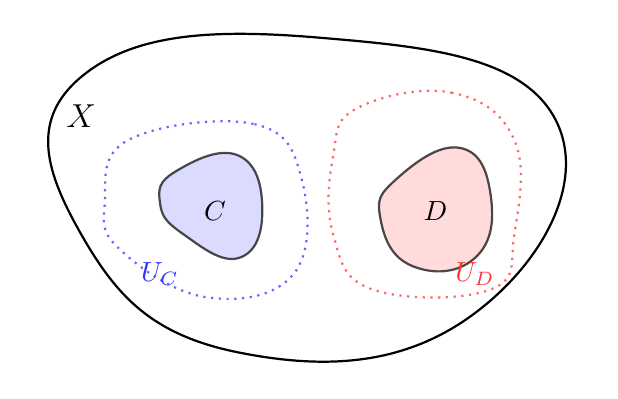
\begin{tikzpicture}[
          closed/.style={draw, thick, fill=gray!40, opacity=0.7},
          open/.style={draw, dotted, thick}
      ]

      % Draw the topological space X
      \draw[thick] plot [smooth cycle, tension=0.8] coordinates {(0,1) (3,1.5) (6,0.5) (5,-2) (2,-2.5) (0,-1)};
      \node[font=\large] at (0,0.5) {$X$};

      % Draw the first closed set C
      \draw[closed, fill=blue!20] plot [smooth cycle, tension=0.8] coordinates {(1.2,-0.2) (2,0) (2.3,-0.7) (2,-1.3) (1.3,-1) (1,-0.6)};
      \node at (1.7,-0.7) {$C$};

      % Draw the second closed set D
      \draw[closed, fill=red!20] plot [smooth cycle, tension=0.8] coordinates {(4,-0.3) (4.8,0.1) (5.2,-0.5) (5,-1.3) (4.2,-1.4) (3.8,-0.8)};
      \node at (4.5,-0.7) {$D$};

      % Draw the open set containing C
      \draw[open, blue!60, thick] plot [smooth cycle, tension=0.7] coordinates {(0.6,0.2) (2.2,0.4) (2.8,-0.3) (2.7,-1.5) (1.6,-1.8) (0.5,-1.2) (0.3,-0.6)};
      \node[blue!80] at (1,-1.5) {$U_C$};

      % Draw the open set containing D
      \draw[open, red!60, thick] plot [smooth cycle, tension=0.7] coordinates {(3.5,0.6) (4.7,0.8) (5.5,0.2) (5.5,-1) (5.2,-1.7) (3.7,-1.7) (3.2,-1) (3.2,0)};
      \node[red!80] at (5,-1.5) {$U_D$};

      \end{tikzpicture}
      \caption{Normal space.} 
      \label{fig:normal}
    \end{figure}
  \end{definition}

  \begin{theorem}
    Every regular space with a countable basis is normal. 
  \end{theorem}

  \begin{theorem}
    Every well-ordered set $X$ is normal in the order topology. 
  \end{theorem}

  \begin{theorem}[Urysohn Lemma]
    Let $X$ be a normal space, and let $A, B$ be disjoint closed subsets of $X$. Let $[a,b]$ be a closed interval in the real line. Then there exists a continuous map
    \begin{equation}
      f: X \longrightarrow [a,b]
    \end{equation}
    such that $f(x) = a$ for every $x \in A$ and $f(x) = b$ for every $x \in B$. 
  \end{theorem}

  \begin{definition}[Separation by Continuous Function]
    If $A$ and $B$ are two subsets of the topological space $X$, and if there is a continuous function $f: X \longrightarrow [0,1]$ such that $f(A) = \{0\}$ and $f(B) = \{1\}$, it is said that \textbf{$A$ and $B$ can be separated by a continuous function}. 
  \end{definition}

  More colloquially, the lemma states that if every pair of disjoint closed sets in $X$ can be separated by disjoint open sets, then each such pair can be separated by a continuous function. 

  \begin{theorem}[Tietze Extension Theorem]
    Let $X$ be a normal space and let $A$ be a closed subset of $X$. 
    \begin{enumerate}
      \item Any continuous map of $A$ into the closed interval $[a,b] \subset \mathbb{R}$ may be extended to a continuous map of all $X$ into $[a,b]$. 
      \item Any continuous map $A$ into the reals $\mathbb{R}$ may be extended to a continuous map of all of $X$ into $\mathbb{R}$. 
    \end{enumerate}
  \end{theorem}

\subsection{Preservation of Normality}

  However, neither products nor subspaces of normal spaces are necessarily normal. 

\subsection{Completely Regular Spaces}

  \begin{definition}[Completely Regular Spaces]
    A space $X$ is \textbf{completely regular} if one-point sets are closed in $X$ and if for each point $x_0$ and each closed set $A$ not containing $x_0$, there is a continuous function $f: X \longrightarrow [0,1]$ such that $f(x_0) = 1$ and $f(A) = \{0\}$. 
  \end{definition}

  \begin{theorem}
    A subspace of a completely regular space is completely regular. A product of completely regular spaces is completely regular. 
  \end{theorem}

  \begin{theorem}
    If $X$ is completely regular, then $X$ can be imbedded in $[0,1]^J$ for some $J$. 
  \end{theorem}

  \begin{corollary}
    Let $X$ be a space. The following are equivalent: 
    \begin{enumerate}
      \item $X$ is completely regular. 
      \item $X$ is homeomorphic to a subspace of a compact Hausdorff space. 
      \item $X$ is homeomorphic to a subspace of a normal space. 
    \end{enumerate}
  \end{corollary}


